%!TEX root = cscw2019-comic.tex
\section{Discussion}
\label{sec:Discussion}
We will first summarize our findings and discuss experimental variations. Then, we will propose a framework for algorithmically synthesizing persuasive messages into the abstract comic form, discuss design implications, and identify limitations.

\subsection{Experiments: Findings and Alternative Contexts}
\label{sub:Experiments: Findings and Alternate Contexts}

From asking individuals to act to appealing for charitable donations, text messages have been widely used in simulating behaviors. Scholars from psychology have shown how variations in the text messages construction alter decisions. In this study, we explored and examined the role of the abstract comic form, a highly expressive, affective medium in communicating persuasive messages. To test the effectiveness of abstract comic persuasive messages, we persuaded individuals to make online charitable donations, a common public good dilemma. In public good dilemma, due to the non-exclusive and non-rivalrous nature of public goods, persuading individuals to contribute is hard and crucial. Also, online charitable donation tasks not only avoid confounding factors such as habit formation which exists in other persuasion tasks (e.g., exercise and healthy diet) but also assure the ecological validity of our study as charity and organizations often solicit donations online. In our study, we compared the persuasive power of text messages, comic messages, and comic messages with social proof in asking charitable donations to public health research (e.g., the Organization for Autism Research).

\begin{description} [leftmargin=\parindent,topsep=0pt,partopsep=3pt,parsep=0pt,itemsep=3pt, listparindent=\parindent]
    \item[Comic vs. Plain Text:] Our results show that study participants prefer persuasive messages in abstract comic form over plain text. When making the charitable donation between $\$0$ to $\$5$, study participants donated $\$ 0.86$ more if they read the persuasive message in an abstract comic form (see~\Cref{fig:robustcontrasts}, fourth column). The results demonstrated the persuasive power of abstract comic in stimulating behaviors in pro-social decisions. Our findings are consistent with prior research on visual persuasive messages and the benefits of comics in communication. One potential explanation is that study participants were more attracted by the comic strip and projected themselves onto the character. When the projection happened, the persuadee may be able to digest the information better which stimulated them to donate more to the Organization for Autism Research. 
    
    \item[Social Proof Condition:] When comparing between the comic condition and comic with the social proof condition, although study participants who read the comic with social proof donated more on average (\$0.19 more) than the comic only condition, our analysis results do not indicate a significant difference between the two conditions (see~\Cref{fig:robustcontrasts}, third column). There are two potential explanations. First, it is possible that the design of our comic strip did not strongly signify the idea of social proof --- we simply introduced the statistic from our pilot study in the text bubble. Other comic designs, e.g., adding other donators as comic characters, may make the social proof more salient. Another potential explanation is that the influence from other study participants is not strong enough. As \textcite{goldstein2008room} discovered in the hotel towel re-use study, the stronger the relationship between the subject and the reference group of individuals is, the more persuasive the message is. The relationship between people on Amazon Mechanical Turk are likely to be weaker than the hotel guests in \textcite{goldstein2008room}'s towel re-use study.

    We conjecture that using a person's social network as part of the social proof (after seeking consent, for example, to use the person's Facebook profile information) may increase the contribution, but needs further research. We know from Cialdini's seminal work on persuasion that the knowledge of friends performing similar behavior is persuasive. We also know from \textcite{small2007sympathy}'s work on charitable donation that named entities are more powerful in persuasion than abstract statistics (e.g. ``Jane Doe is a hurricane survivor; please help'' vs. ``3000 people homeless due to the hurricane; please help''). If the person has given consent, a charity could find out in real time, the Facebook friends of the person who have loaded the web-page, and compute the fraction who have donated and use that number in the social proof. Or a charity can use tie-strength \cite{Gilbert}, if available, and name the closest friend who has donated to the charity in the social proof message. However, it may backfire as we know from recent work \cite{eslami2018communicating} that when advertisers display information that subjects find ``creepy'' (as demonstration of knowledge by the charity of the subject's closest friend, of even statistics of the person's Facebook friends circle contributions), the subjects may find the charity less trustworthy and may donate less.
    
    \item[Donation Amount:] Another natural question to ask is whether the maximum donation amount of  \$5  in our study has any influence on our findings (e.g., will people make the same donation decision if they can donate more?).  Prior studies in behavioral economics suggested that small-stake experiment in developed countries can be replicated in developing countries where the stake becomes a significant portion of participants' weekly income \cite{binswanger1980attitudes,binswanger1981attitudes,kachelmeier1992examining}. Additionally, \textcite{post2008deal} showed that the results from small-stake experiments would hold with higher stakes in developed countries as well. Those results seem to suggest that our findings will hold with higher donation amount. However, the best way to confirm is through actual experiments. 
    
   \item[Other Media Forms:] While a direct comparison between the abstract comic form and other visual forms such as image and video is beyond the scope of the paper, we discuss two advantages of using the abstract comic to persuade. There are two points to consider: the ease of making a connection with a viewer (the abstract comic form vs. images or video); the infrastructure to create tailored messages. First, as \textcite{mccloud2011making} points out, when using the abstract comic form, the reader projects themselves onto the character whereas a concrete and detailed representation of the person in the comic can cause the reader to develop a sense of the ``other'' - that is, they are viewing someone else enacting a scene. Images and videos often use actual human models which will create a sense of the ``other'' for the viewer. So, images/videos need to connect with the viewer through other demographic, cultural and local cues. For example, in advertising, to allow recipients of ads to identify or resonate with the message context, advertisers try to ensure that the models who appear in images match the target demographic. In contrast, when viewing an abstract comic, readers fill in the gaps with their own characteristics, and they see themselves as the protagonist. Second, our infrastructure (discussed next in~\Cref{sub:framework}) makes it straightforward for a charity to compose a multi-panel abstract comic. The infrastructure to create tailored imagery and videos may be expensive for the charity. Today, advertisers tailor the imagery (usually the individual in the image) in online banner ads (embedded on a web page) to the demographics of the person viewing the ad. Matching the demographics requires that advertisers access the information stored in a browser cookie against third-party information about the person in real-time. This real-time switching of imagery is expensive: it requires a manually curated image collection corresponding to individuals matching to different demographic segments of interest. And, to personalize the message (e.g. with the social proof), they would need to have the infrastructure to compose the message on the fly. Furthermore, algorithmic synthesis of persuasive, personalized videos is more challenging. One possibility that we do consider as part of future work: animations that involve the abstract comic form.

    \item[Experiment Flow in the Real World:] We consider three online charitable donation scenarios related to how the charitable organization knows the person asked to make a donation. In each case, consistent with prior work ~\cite{pessemier1977willingness}, the charity needs to establish context.
    
    First, the person may be familiar with the charity through their lived experience. For example, in the case of Wikipedia, the person may use the site frequently. A person who regularly uses the Wikipedia site is unlikely to need a video describing Wikipedia benefits. In such cases, we envision using the three-panel comic instead of the desktop banner ad that Wikipedia uses at the moment.
    
    Second, the person may be a member of a charity or a non-profit organization (e.g. museums). For non-profit organizations with memberships, they can recognize a member has logged onto the organization website. In this case, detailed context may be less necessary and organizations could use the three-panel comic in their regular donation page, along with social proof describing the fractions of other members who have contributed.
    
    Third, the person may not know the charity. For charities who need to ask for donations from people without neither lived experience nor memberships, they need to establish context from scratch. They may establish context through videos, a page with text and images or even a physical mailer. After watching the videos or reading the page, they may show the person a comic message. For the physical mailer, the charity would include its usual textual description and imagery followed by the abstract three-panel comic. After the comic panel, they may direct the person opening the mailer make a contribution on a web-page.
    
    For the first two scenarios, a charitable organization (e.g. Wikipedia) can determine regular use of its website or determine if the person visiting the web-page is an organization member through the use of advertising cookies with permission.

\end{description}

 \subsection{Framework for Algorithmically Synthesized Abstract-Comic Persuasive Messages}
 \label{sub:framework}
 
Our study showed the persuasive power of abstract comics in encouraging people to make pro-social decisions. However, one drawback of using visual stimulus in persuasion is the cost during creation processes. Although compared to creating other persuasive visual stimuli such as videos or complex graphical illustration, due to its simplicity, abstract comics requires much less effort. In this section, we propose a framework that allows full/semi- automatic generation of abstract persuasive messages and identify crucial features that need to be addressed in future work. We believe such a tool will lower the barrier for the persuader to take advantage of the abstract comic (as demonstrated in our study) in encouraging individuals to act in public good dilemmas.

In our study, we created a comic generator with existing packages including ``cmx.io'' \cite{cmx.io} and ``rough.js'' \cite{rough.js} to generate three-panel abstract comic strips. With several pre-defined character gestures (see~\Cref{figur:figures}), the generator only requests the text input from the persuader to create the comic message.  

We believe the comic generator built in this study can be further developed as a framework for algorithmic synthesis. Now, we identify crucial features that need to be addressed in future research. First, the framework should be able to automatically select the character gesture that best fits the persuasive message's context. For example, when the message receiver was told good news, his/her gesture should reflect that conflict. The appropriate mapping will create a natural and coherent comic message which is the key for an expressive message. We need future research to realize such a method. Second, the framework should be able to use other comic elements, such as inter-character distance and shading, to create persuasive comics. To achieve this feature, we need to understand how different elements affect the persuasiveness of the abstract comic messages. Third, the framework should be able to personalize the persuasive comics by using persuadee's behavioral data to inform comic contents. We could derive the statistics for the social proof from the behaviors of a person's friends and the data from his/her own activities.


\begin{figure}[t]
    \centering
    \begin{tabular}{cc}
        \subfloat[Gestures for positive framed messages]{\label{figur:1a}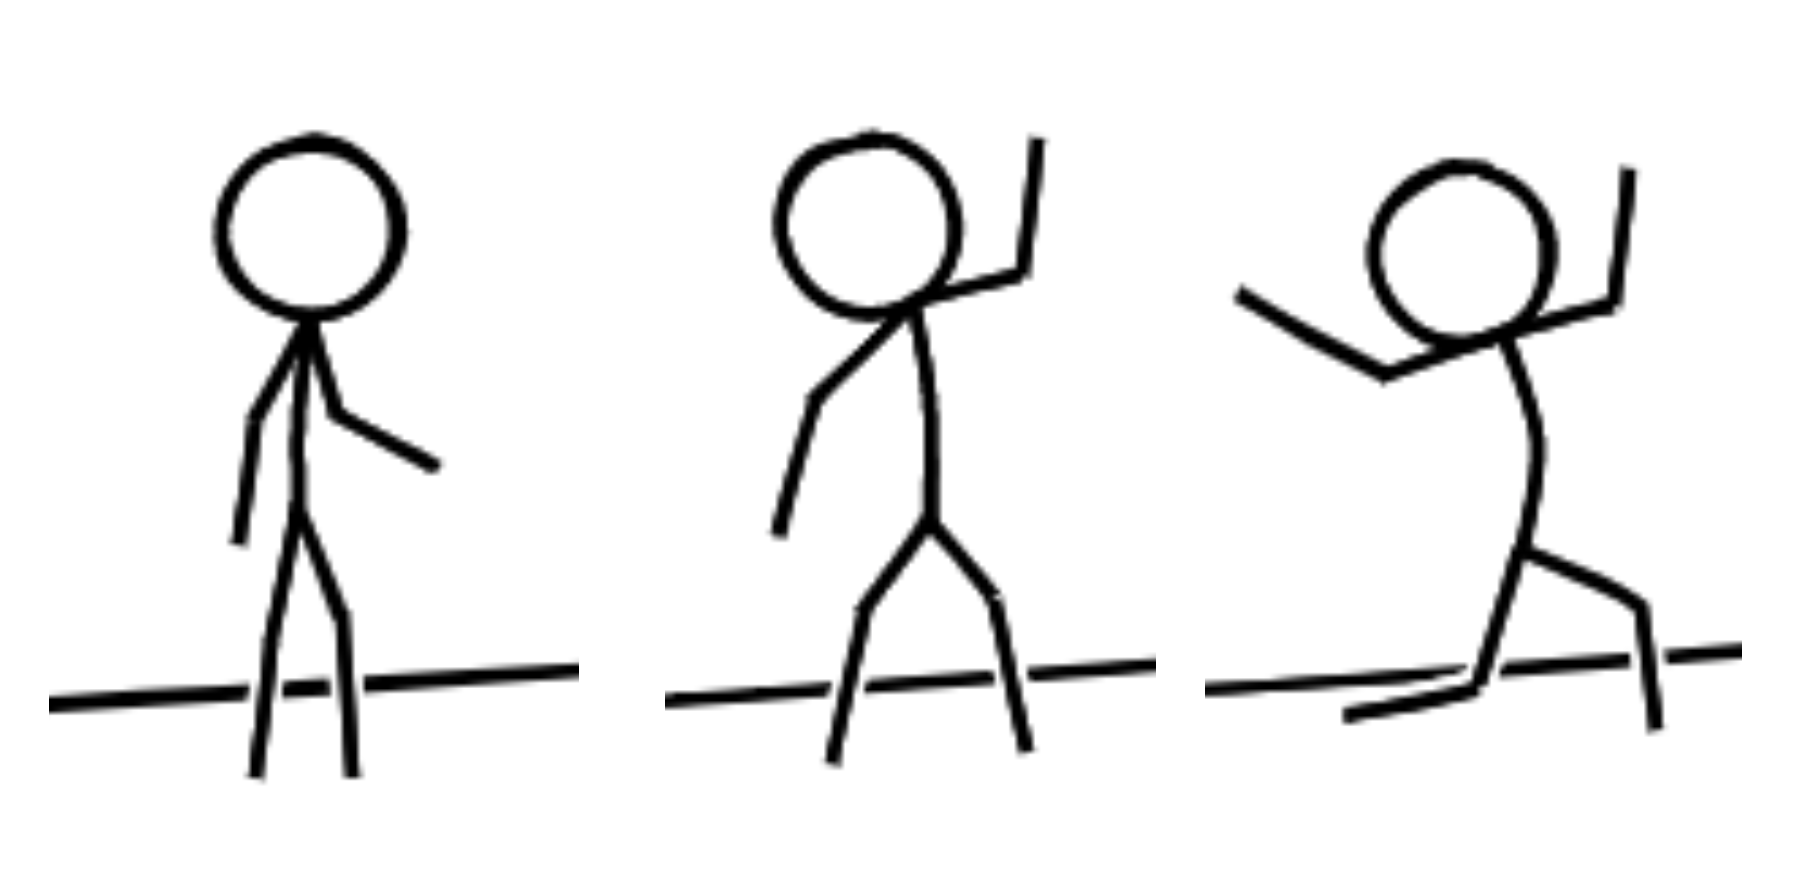
\includegraphics[width = 0.4\columnwidth]{figures/pos_figures}} &
        \subfloat[Gesture for negative framed messages ]{\label{figur:1b}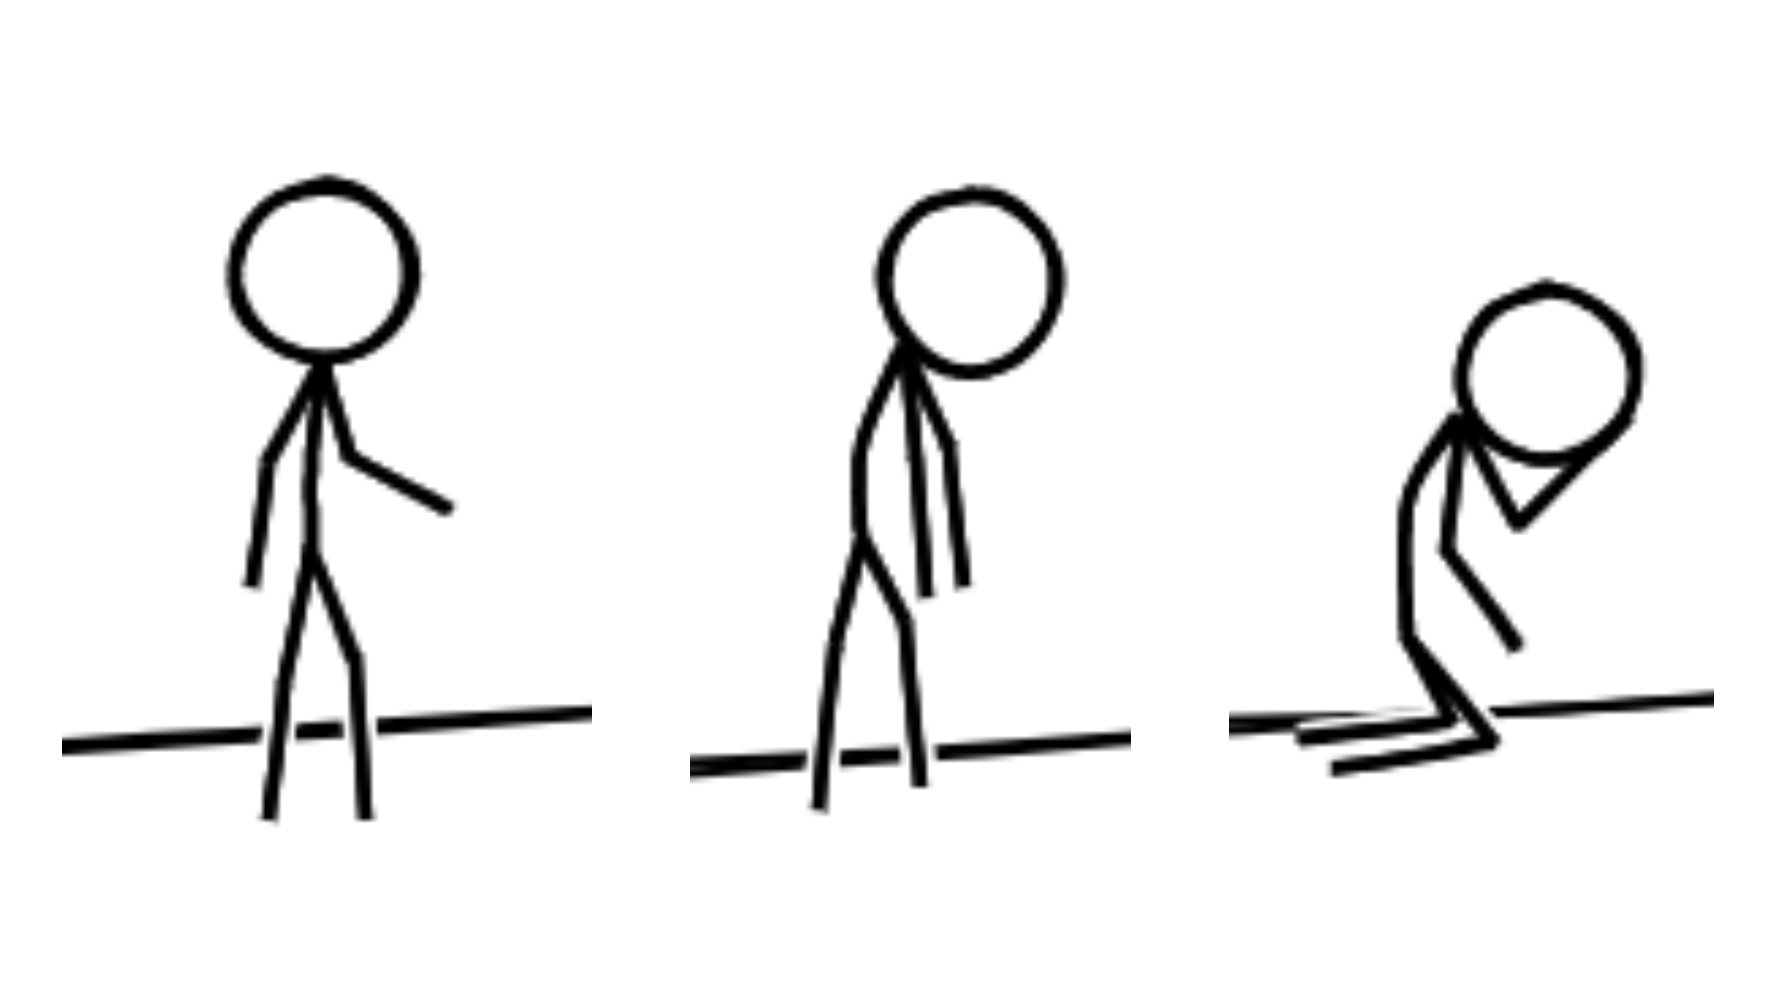
\includegraphics[width = 0.4 \columnwidth]{figures/neg_figures}}\\
    \end{tabular}
    \caption{Different character gestures to communicate various levels of emotional intensity. The left figure shows gestures from neutral to the happiest. The right figure shows gestures from neutral to the most frustrated. }
    \label{figur:figures}
\end{figure}

\subsection{Design Implications}
Our main design implications are two-fold. First, when encouraging individuals to contribute to public goods, non-profit organizations and governmental agencies ought to consider using abstract comic in their online messaging campaign to persuade. From our results, using abstract comics can, in particular, persuade people to act in public-goods dilemmas that require single-shot decisions (online charitable donations). Additionally, when constructing persuasive comics, it is worthwhile to consider to incorporate social proofs. In the study, the purpose of the video is to inform participants about the context. Charities could use the comic after they've established context as discussed in~\Cref{sub:Experiments: Findings and Alternate Contexts}. 

Second, our results also inform the development of a computational framework that can algorithmically synthesis textual persuasive messages into abstract comic form and use data-driven methods to personalize the message to further increase messages' persuasive power. 

\subsection{Limitations \& Future Work}
\begin{description}[leftmargin=\parindent,topsep=0pt,partopsep=3pt,parsep=0pt,itemsep=3pt, listparindent=\parindent]
\item[Distant and Non-exclusive Task:]  Although our study asked participants to make the decision with a real cost, the decision domain is limited to only one scenario, online charitable giving. In this task, the participant's reward is distant and non-exclusive (e.g., participant's donation decision won't bring any immediate reward and won't exclude the participant from the research outcome). Although both characteristics help us clearly test the persuasive benefits of abstract comics, they limited our generalizability. We need future research to understand the pros and cons of using abstract comic messages in persuasive tasks with different reward characteristics. For example, for persuasive goals in the quantified-self movement~\cite{Epstein2014,Choe2014} such as exercise and dieting, the reward is distant (e.g., people's health won't be improved immediately after exercise) but exclusive (e.g., healthy life situation mainly benefit the individual him/herself). Moreover, our persuasion task is for an online charitable donation. Future work is needed to extend our result to offline charitable donation solicitation where persuasive text messages, such as mailers, also often used. 

\item[Study on Amazon Mechanical Turk:] Consistent with prior research \cite{lee2013does,saunders2016no,sussman2015framing,arechar2017turking,branas2018gender} that used Amazon Mechanical Turk to study charitable donations, we recruited our participants from Amazon Mechanical Turk.


Although research shows that populations on Amazon Mechanical Turk are diverse and can mirror the US population \cite{buhrmester2011amazon,behrend2011viability,berinsky2012evaluating}, there are concerns about Amazon Mechanical Turk's sample representativeness \cite{landers2015inconvenient,paolacci2010running}. One potential solution is to use panel population where the panel company claimed to offer a more diverse and representative sample.
However, this method also has concerns in that the researcher can not directly cross-validate the sample's representativeness. Another solution is using stratified sampling, but it is challenging to classify every member of the population into a subgroup properly. 

Another limitation from the use of Amazon Mechanical Turk subjects in our study is that prior research \cite{paolacci2010running,paolacci2014inside,kaufmann2011more} indicates that compared to other recruiting methods, study participants from Amazon Mechanical Turk are more sensitive to monetary rewards as the monetary reward is their prime motive for participation. Since we ask our Amazon Mechanical Turk study participants to donate from their own prospective rewards, we may see a lower average donation across all conditions than asking the population sample less sensitive to monetary rewards. An alternative sampling method we could consider in the future work is recruiting participants from our own social network. We conjecture that we may see higher average contributions in each of the three conditions, since participants on social network may be less sensitive to monetary rewards than those on Amazon Mechanical Turk. However, we need to carefully control for other potential confounding factors such as study participant's knowledge about our experiment goal. 

  \item[Comic Message Construction:] In our study, we constructed the comic messages in the XKCD comic style. Although the XKCD style is easily recognizable, there are many different ways to create abstract comics.  Comic, as a creative art form, has rich semantics and vocabularies to communicate ideas \cite{scott1993understanding}. Out of necessity, we limited the complexity our comics strip (e.g., number of characters, gestures, and the number of panels). Future research is needed to explore and understand how other comic elements, for example, inter-character distance and character's gesture, affect the persuasiveness of the comic. Furthermore, while simplicity grants us the possibility to automate the generation process, future technology may allow us to generate more complicated persuasive abstract comics.
  
    \item[Other Experimental Contexts:] What are other contexts to which our study results may apply? Although our study examined charitable donation decisions, a single shot task with distant, non-exclusive rewards, certain health related tasks may be candidates to study next. Recent work by~\textcite{Bushar2017} on using SMS text messages to persuade pregnant mothers to take influenza vaccinations suggests that those who received the text messages were more likely to report taking a vaccination than those who did not receive a message. Further research will be merited to determine if for this single-shot task, with exclusive, non-immediate reward, an abstract comic (e.g. embedded as a link in the SMS) succeeds in increasing vaccination rates for pregnant women over the plain text.
  
\end{description}